\begin{frame}
    \frametitle{P2P Network}
    The steps to run the network are as follows:
    \begin{itemize}
        \item New transactions are broadcast to all nodes.
        \item Each node collects new transactions into a block.
        \item When node finds a proof-of-work, it broadcast the block to all nodes.
        \item Nodes accept the block only if all transactions in it are valid and not already spent.
        \item Nodes express their acceptance of the block by working on creating the next block in the chain, using the hash of the accepted block as previous hash.
    \end{itemize}
\end{frame}

\begin{frame}
    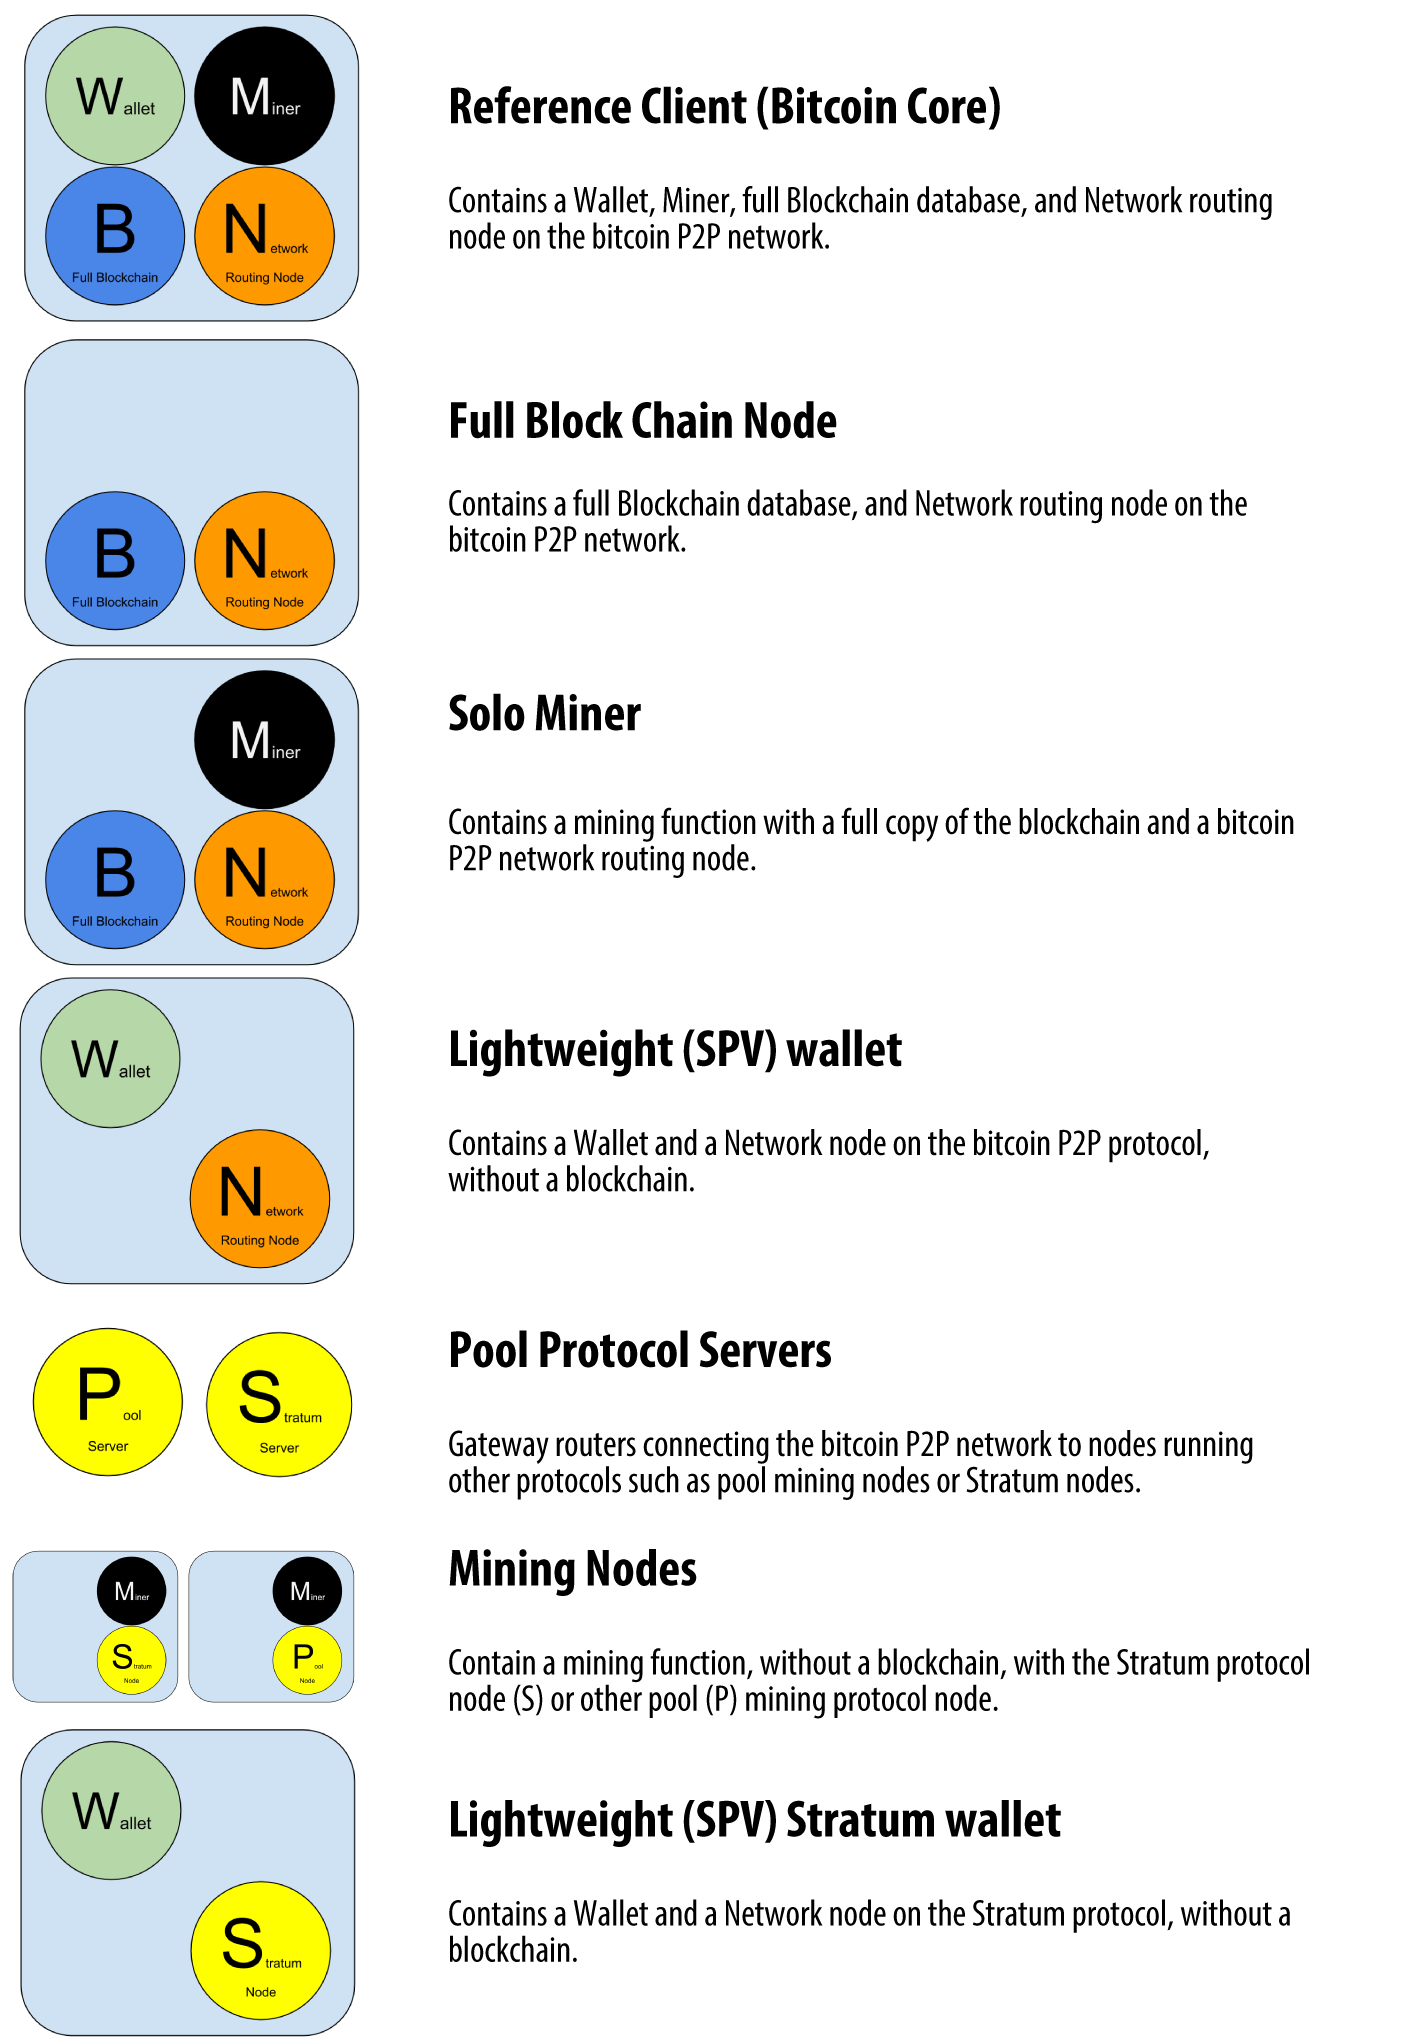
\includegraphics[scale=0.6]{mbc2_0802.png}
\end{frame}

\begin{frame}
    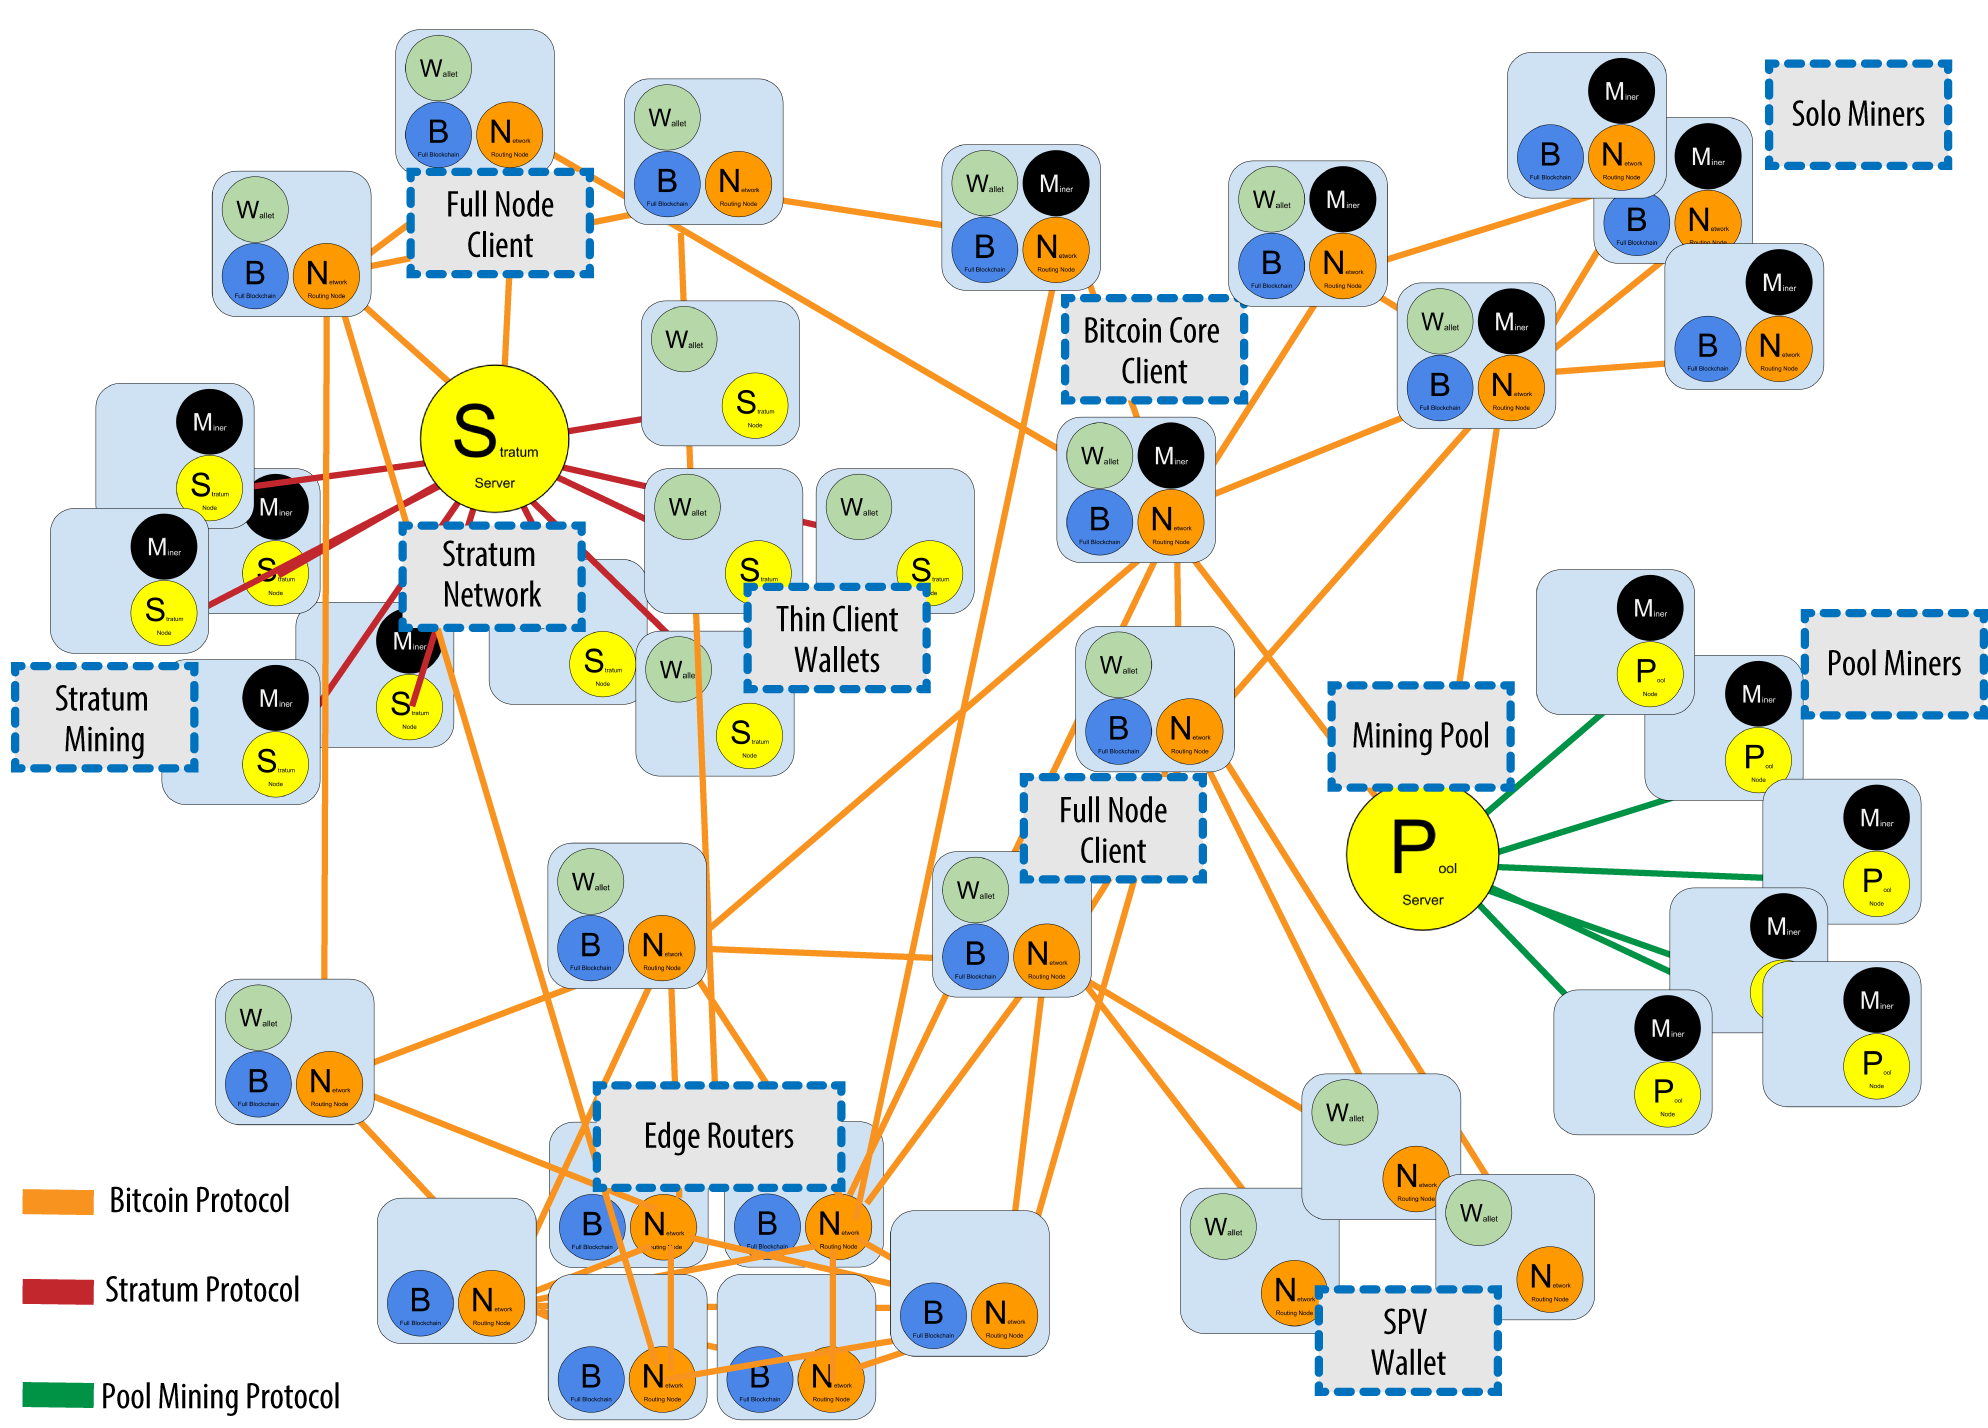
\includegraphics[scale=0.15]{mbc2_0803.png}
\end{frame}
